\documentclass[12pt]{article}
\setlength\parindent{0pt}
\usepackage{fullpage}
\usepackage{amsmath}
\usepackage{hyperref}
\usepackage{graphicx}
\usepackage[margin=1.5cm]{geometry}
\setlength{\parskip}{4mm}
\def\LL{\left\langle}   % left angle bracket
\def\RR{\right\rangle}  % right angle bracket
\def\LP{\left(}         % left parenthesis
\def\RP{\right)}        % right parenthesis
\def\LB{\left\{}        % left curly bracket
\def\RB{\right\}}       % right curly bracket
\def\PAR#1#2{ {{\partial #1}\over{\partial #2}} }
\def\PARTWO#1#2{ {{\partial^2 #1}\over{\partial #2}^2} }
\def\PARTWOMIX#1#2#3{ {{\partial^2 #1}\over{\partial #2 \partial #3}} }
\newcommand{\BE}{\begin{displaymath}}
\newcommand{\EE}{\end{displaymath}}
\newcommand{\BNE}{\begin{equation}}
\newcommand{\ENE}{\end{equation}}
\newcommand{\BEA}{\begin{eqnarray}}
\newcommand{\EEA}{\nonumber\end{eqnarray}}
\newcommand{\EL}{\nonumber\\}
\newcommand{\la}[1]{\label{#1}}
\newcommand{\ie}{{\em i.e.\ }}
\newcommand{\eg}{{\em e.\,g.\ }}
\newcommand{\cf}{cf.\ }
\newcommand{\etc}{etc.\ }
\newcommand{\Tr}{{\rm tr}}
\newcommand{\etal}{{\it et al.}}
\newcommand{\OL}[1]{\overline{#1}\ } % overline
\newcommand{\OLL}[1]{\overline{\overline{#1}}\ } % double overline
\newcommand{\OON}{\frac{1}{N}} % "one over N"
\newcommand{\OOX}[1]{\frac{1}{#1}} % "one over X"



\begin{document}
\Large
\centerline{\sc{Homework 2}}

\pagenumbering{gobble}

\begin{center} \normalsize Due Thursday or Friday, 2 or 3 February, at the beginning of recitation. 
\end{center}
\normalsize

\it This homework set is specifically designed to prepare you for Exam 1, held on 7 February. All of the problems here touch on ideas that you may need for the quiz. 

If you have a cat, dog, bird, horse, lizard, snake, or pet rock you'd like to see featured in a homework set or exam problem, send me their picture along with what they like to do!

\rm
\begin{enumerate}

\item Part 4 of Question 2 asks you to compute the acceleration of an object, given the change in position, the initial velocity, and the final velocity. To do this, you will need to use both $x(t)$ and $v(t)$ kinematics equations, but ultimately you will eliminate the variable $t$.

Often in mechanics we aren't particularly concerned about time -- we're only concerned with the change in position, initial velocity, final velocity, and acceleration.
These are related by the ``third kinematics equation'', 

$$
v_f^2 - v_0^2 = 2a(x_f - x_0)
$$

Show that this equation is simply a consequence of the other two.

{\it Algebra hint:} Starting from the $x(t)$ and $v(t)$ formulae for constant acceleration, solve one equation for $t$ and substitute it back into the other one. (The algebra here is very similar to Week 2 Day 1's recitation, second problem.)

\bigskip

\item Matthew Todd, one of the physics department students, has a dog named Walter. (I'm not named after him, sadly -- he's a great dog!) 

\begin{minipage}{0.55\textwidth}Matt is teaching him about two-dimensional motion. He's very good at it already -- but only if it involves his favorite tennis ball.

\bigskip

Matt and Walter are out on the grass in the Quad, $d=20$ meters apart. Matt throws the ball directly to him to catch at an angle of $theta=55^\circ$ above the horizontal. He's an accurate thrower, so the ball goes right to Walter -- he doesn't have to run to catch it. 

\begin{enumerate}
	\item What speed did Matt have to throw the ball at for Walter to catch it?
	\item How long was the ball in the air?
	\item How fast was the ball traveling when it was at the apex of its flight?
	\item Suppose that his arm moved through a distance $b=80$ cm while pushing the ball forward before he released it at the speed you calculated in part (a). What acceleration would he have to impart to the ball while throwing it?
\end{enumerate}
\end{minipage}
		\begin{minipage}{0.45\textwidth}
	\begin{center}
		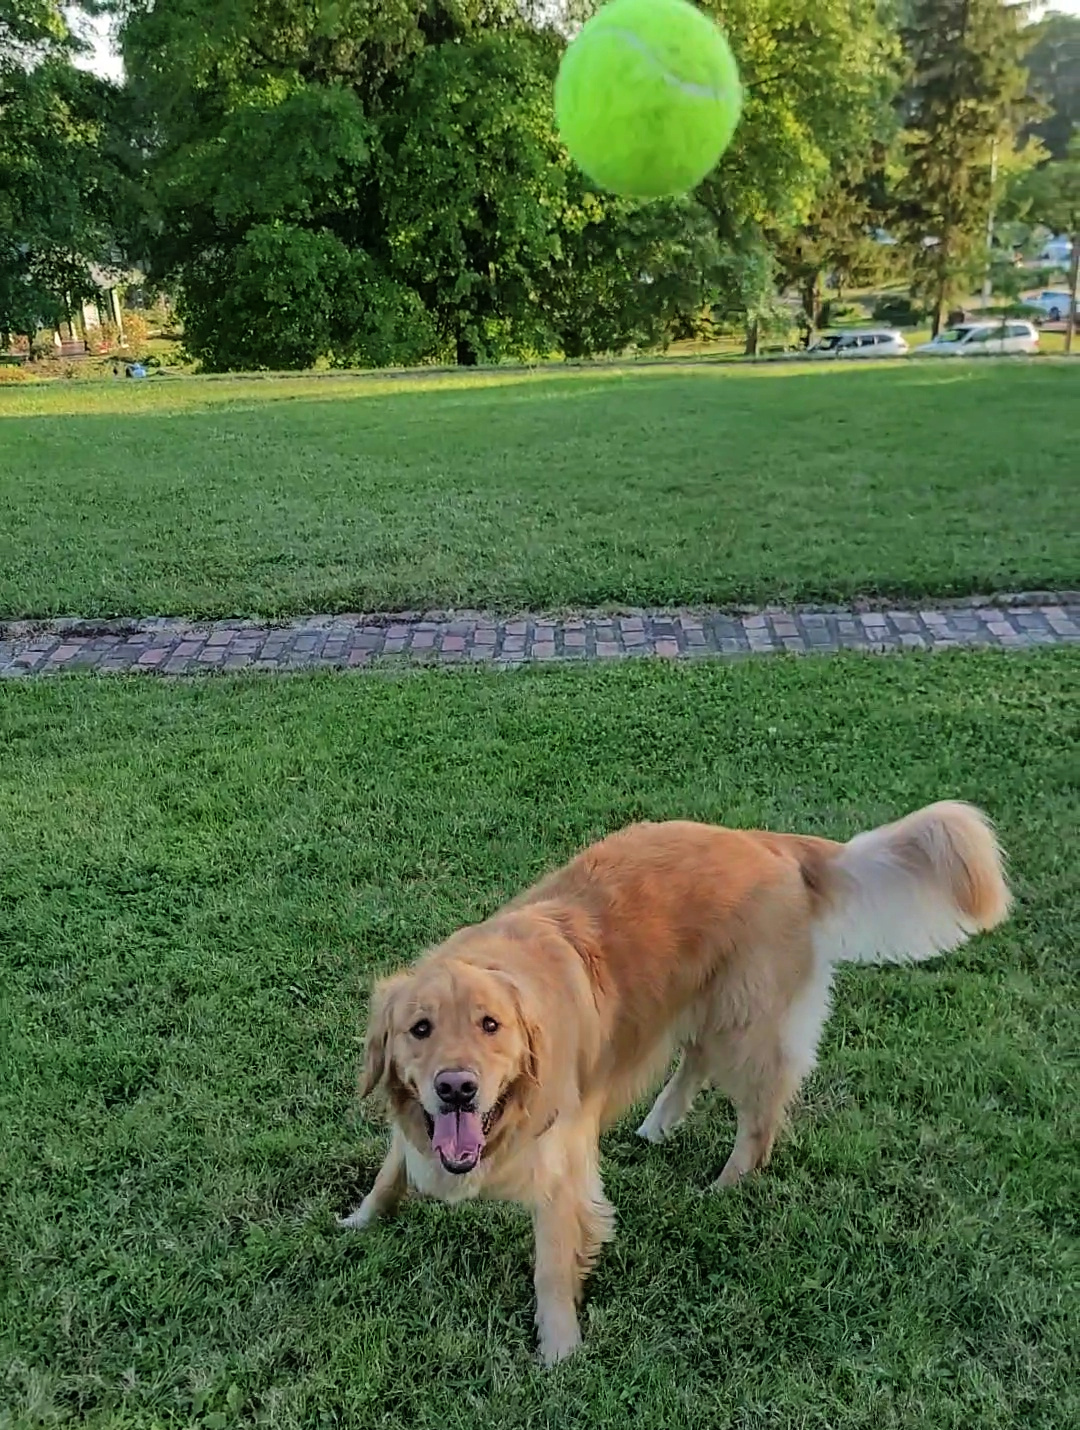
\includegraphics[width=0.9\textwidth]{walter.jpg}\\
		\scriptsize \it 
		He will eat your homework if you don't play with him!
	\end{center}
\end{minipage}

\bigskip


\item Our previous head TA, Mario Olivares, has an adorable dog named Teddy. 
\bigskip

	\begin{minipage}{0.5\textwidth}

	Suppose Mario throws a ball out into the lake for Teddy to catch. It lands $d=7$ meters out into the water. Teddy is standing on a flat platform 2 meters above the water. Wanting to get his ball back, he runs down the 
		platform and flies out over the water, landing on top of his ball. Suppose that Teddy runs straight off the platform, so that he is moving horizontally when he leaves the ground.

\begin{enumerate}
\item How fast was Teddy moving when he left the platform? 
\item How fast was Teddy moving when he landed in the water?
\item In what direction was Teddy moving when he splashed into the lake? (Give your answer in a physically meaningful way: ``X degrees below the horizontal" or similar.
\end{enumerate}

	\end{minipage}
		\begin{minipage}{0.5\textwidth}
			\begin{center}
				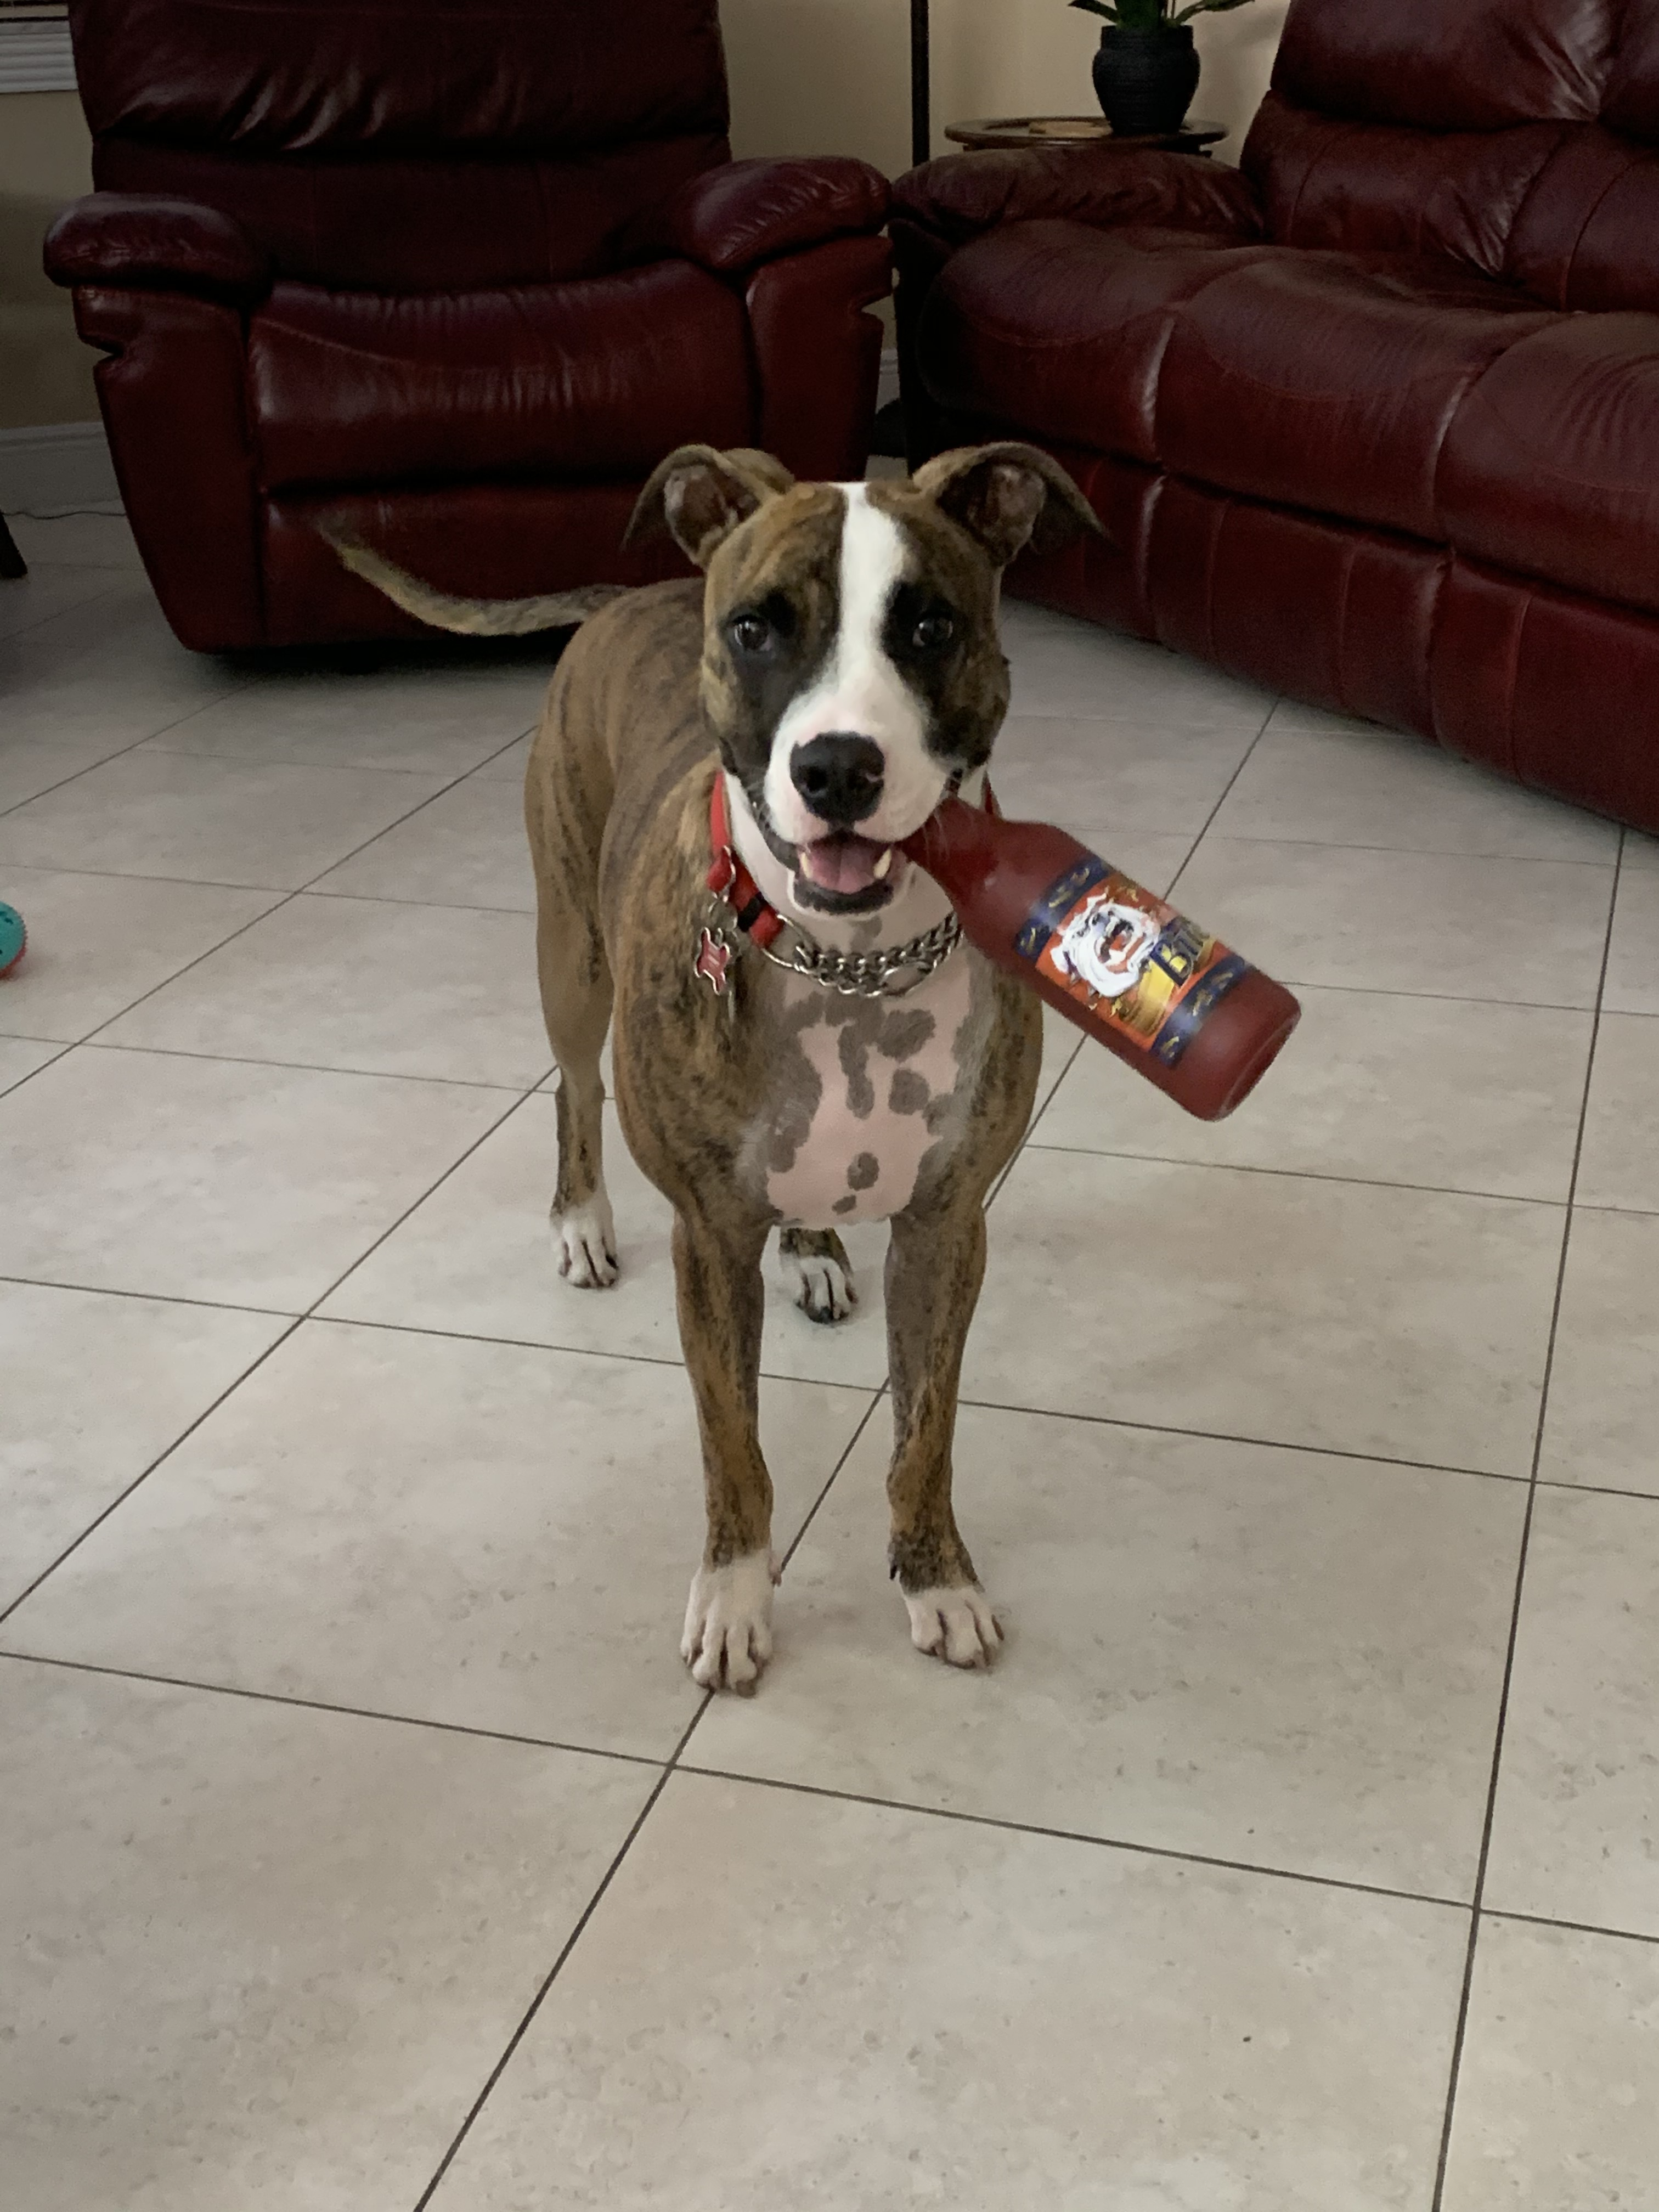
\includegraphics[width=0.9\textwidth]{teddy.jpg}
			\end{center}
		\end{minipage}


\bigskip
\bigskip

\item One of our former coaches adopted a tiny little one-eyed kitten named Mary last year. 

\bigskip
\begin{minipage}{0.45\textwidth}

	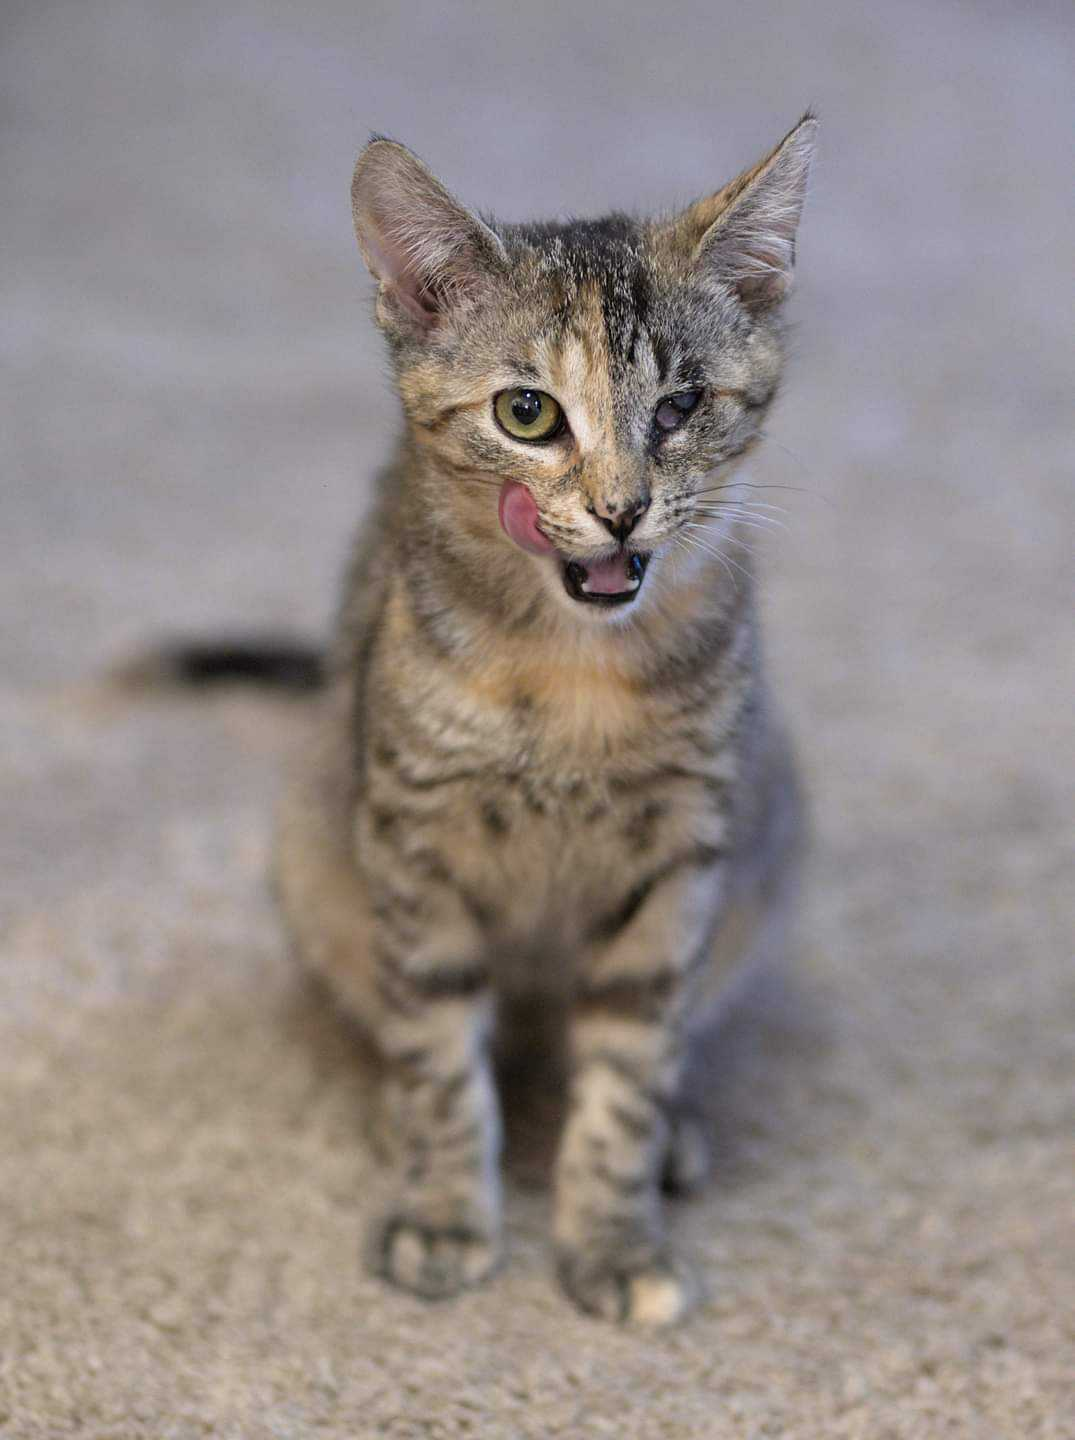
\includegraphics[width=0.9\textwidth]{mary1.jpg}
\end{minipage}
\begin{minipage}{0.55\textwidth} Mary was rescued from a barn and is very athletic. She can jump 120 cm off of the ground (and uses this talent all the time to jump up on tables where she thinks she can steal someone's dinner...) This means that she can push herself off the ground with enough velocity to reach a height of 120 cm. {\it (Note that this velocity is a property of Mary herself; no matter where we take her, this velocity is the same.}

\begin{enumerate}
\item With what velocity must Mary leave the ground in order to jump 120 cm high?
\item How long will she be in the air before she lands?
\end{enumerate}
\end{minipage}
\newpage


\item Suppose that her owner now takes Mary to an elevator, accelerating upward at $\alpha=2\, \rm m/\rm s^2$. Mary jumps up and tries to swat one of the elevator buttons. This elevator button is 110 cm above the floor of the 
	elevator.

\begin{enumerate}
\item If Mary jumps as high as she can, will she be able to push the button? How far above the elevator floor will she make it?
\item How long will Mary be in the air?
\end{enumerate}

{\it Hint: Think very carefully about your coordinate system, and all of the consequences of the accelerating elevator. You may need the quadratic formula for this problem. If you are still stuck, draw position vs. time graphs for 
		both Mary and the elevator button on the wall that she is trying to push.}


\item She then travels to the planet Twilo with her kitten, which is quite Earthlike except for its value of $g=11.8\, \rm m/\rm s^2.$

\begin{enumerate}
\item How high can Mary jump on Twilo?
\item Based on a comparison of the last two problems, can you make any statements regarding gravity and acceleration?
\end{enumerate}

%\item An object's position is given by the vector 
%
%$$\vec s(t) = (3\,\rm m/\rm s^3) t^3 \hat i + (4\, \rm m/\rm s^2) t^2 \hat j + (8\, \rm m/\rm s) t\hat k.$$
%
%\begin{enumerate}
%\item What is its velocity as a function of time?
%\item What is its acceleration as a function of time?
%\item Where is it at $t=10$ s?
%\end{enumerate}


\bigskip


%\item An object's position is given by the vector 
%
%$$\vec s(t) = (2\, \rm m) \cos (\omega t) \hat i + (2\, \rm m) \sin (\omega t) \hat j$$
%
%where $\omega = 1$ radian per second.
%
%\begin{enumerate}
%\item How would you describe this object's motion? What shape is it moving in?
%\item \it Hint: if you are stuck, compute and graph its position in the Cartesian plane at a variety of values of t (say, for integers 0-6).
%\end{enumerate}
%
%
%\bigskip


\item A hiker is standing on the top of a mountain with a slope of 45 degrees. They kick a rock horizontally off of the top of the mountain at an initial speed $v_0$; it sails through the air until it lands 
	lower on the slope.

	\begin{enumerate}
		\item Think very carefully about how you can describe ``The rock lands back on the slope'' in mathematical terms. It will help to draw a picture, as always.
		\item Where on the slope does the rock land?
	\end{enumerate}

\end{enumerate}
\end{document}

